\chapter{Implementierung der Webadministration}
\label{cha:impl_web}

Die Web Administration stellt die zentrale Kontrolleinheit des gesamten Projekts dar. Über die Web Administration werden sämtliche Einträge der Datenbank verwaltet, dies schließt neben der Benutzer- und Geräteverwaltung ebenfalls die Verwaltung aller Regale und Produkte ein.


\section{Technologische Grundlagen}

Die Administrationsoberfläche ist als Webapplikation und im Speziellen als Single-Page-Applikation konzipiert, d.h. sie besteht grundlegend aus einer einzigen Webseite, deren Layout (wie für Webseiten üblich) auf \ac{HTML} und \ac{CSS} aufgebaut ist. Die einzelnen Ansichten (Views) der Anwendung sowie jegliche dynamische Interaktionsprozesse werden über \acl{JS} als clientseitige Scriptsprache gesteuert. Dabei werden auch Daten oder Views im Hintergrund asnychron über \ac{AJAX} nachgeladen. Durch dieses Grundkonzept werden viele Ladevorgänge der kompletten Webseite vermieden und nur die Daten nachgeladen, die im Einzelnen benötigt werden -- dies sorgt für eine bessere Performance der Anwendung und somit eine bessere User Experience.

Das Layout selbst ist \emph{responsive}, d.h. es passt sich flexibel an die gegebene Bildschirmgröße des Ausgabegerätes durch eine optimiertes Layout (veränderte Anordnung von Seitenelementen, optimierte Platznutzung) an. Dadurch ist die Webadministration nicht nur für die Nutzung am Desktop-PC und großen Bildschirmen, sondern auch für die Verwendung auf Tablets und Smartphones gerüstet, sollte die Webanwendung im gesamten Netzwerk verfügbar sein (siehe Architektur).

Wie bereits in der Architektur angedeutet, läuft die Webadministration serverseitig mit der Scriptsprache \ac{PHP}. Hierüber werden Inhalte und Layoutkomponenten vorgeneriert und abhängig von den Parametern der clientseitigen Anfragen ausgeliefert. Auch die Validierung von Formularanfragen, sowie die Verbindung zur Datenbank und Datenbank-Abfragen werden über \ac{PHP} durchgeführt. Für die Datenbank selbst wird wegen der guten Kompatibilität mit PHP auf MySQL gesetzt.

Unter bestimmten Bedingungen (z.B. Sicherheitsvorschriften oder technische Einschränkungen) könnte die Ausführung von JavaScript im Browser des Anwenders nicht möglich sein. Die Webadministration ist in ihrer Funktionalität zu einem großen Teil auch ohne aktiviertes \acs{JS} lauffähig, indem die statischen Fallback-Links und Standardfunktionalitäten greifen, die via JavaScript sonst geblockt und eigene Interaktionsmethoden ersetzt werden. Dennoch lassen sich Teile der Anwendung ohne Einsatz von JavaScript nur sehr aufwändig umsetzen; als Beispiel dafür sei hier der Shelf Designer genannt, der im Folgenden noch näher beschrieben wird und ohne \acs{JS} nicht funktionsfähig ist.


\section{Bereiche und Funktionen}

Das Layout der Webadministration ist in eine Navigationsleiste, eine Subnavigation und einen Inhaltsbereich aufgeteilt. Über die Navigationsleiste können die funktionalen Hauptbereiche geöffnet werden, die jeweils in der Subnavigation noch über Unterseiten verfügen. Der Inhaltsbereich enthält häufig Tabellen, die rechts eine Spalte mit Buttons für Aktionen zu einem Eintrag der Tabelle bereit halten. Tabellen, die wegen einer hohen Anzahl an Einträgen sehr lang werden würden, werden dabei automatisch auf mehrere Seiten verteilt, die über eine dann eingeblendete Seitennavigation geöffnet werden können. Die restlichen Views sind i.d.R. Formulare (z.B. für \emph{Neue Produkt anlegen} oder, bereits vorausgefüllt, \emph{Produkt bearbeiten}).

In den folgenden Kapiteln sollen die Bereiche der Webadministration ausführlich vorgestellt werden. Auf eine detaillierte Aufführung der betroffenen Daten und Felder wird dabei zwecks Übersichtlichkeit verzichtet -- diese wurden bereits in der Datenbank-Architektur (Kapitel \ref{sec:architektur_datenbank}) genauer erläutert.


\subsection{Produkte \& Einheiten}

\begin{figure}[H]
	\centering
	{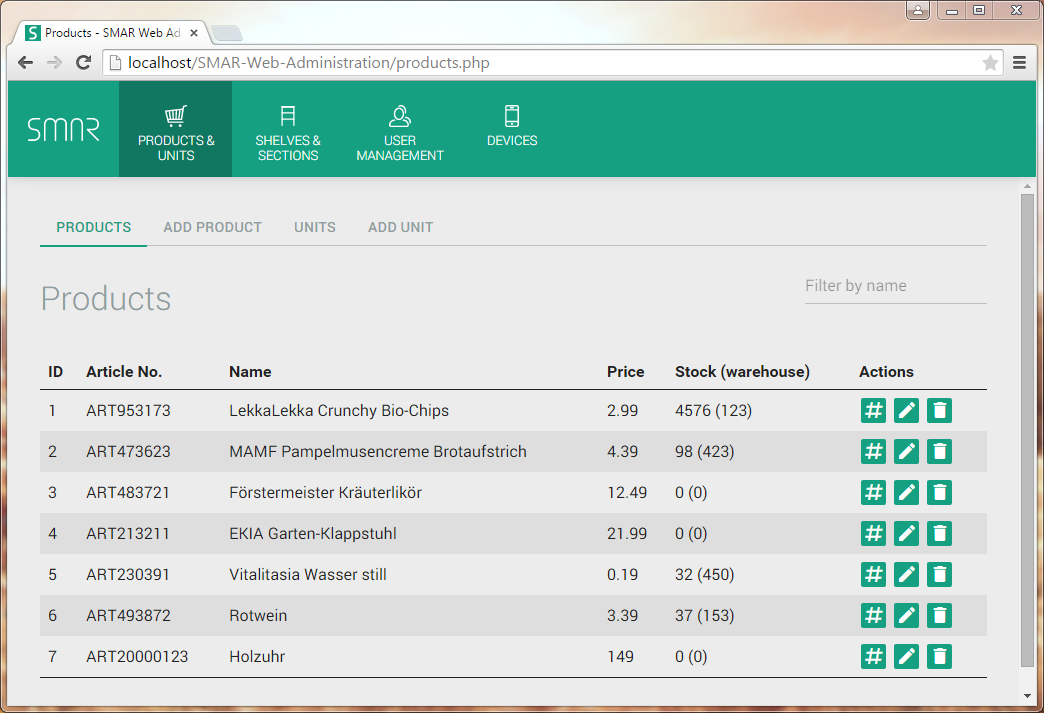
\includegraphics[width=\textwidth]{Bilder/Abbildungen/webadmin_products.png}}
	\caption{Produktübersicht in der Webadministration (Screenshot)}
	\label{fig:webadmin_products}
\end{figure}

In diesem Bereich der Webadministration können alle wesentlichen Aspekte rund um Produkte und die Einheiten, in denen Produkte auftreten können, verwaltet werden.\\

Als erstes wird eine Produktübersicht in Listenform angezeigt, über welche alle vorhandenen Produkte gefunden werden können. Zu einem Produkt werden die wesentlichen Informationen angezeigt, um ein Produkt identifizieren zu können, sowie der aktuelle Warenbestand eines Produktes. Über die Aktionen kann ein Produkt bearbeitet oder gelöscht werden, sowie die entsprechenden Produkt-Einheiten-Mappings angezeigt werden, die im Folgenden noch erläutert werden.\\

Auf einer Unterseite, erreichbar über die Subnavigation, kann über ein Formular ein neues Produkt angelegt werden, indem die notwendigen Informationen angegeben werden. Die notwendigen Abhängigkeiten zu anderen Tabellen werden dabei von der Webadministration automatisch angelegt. Analog gibt es ein Formular zum Anlegen von Einheiten für Produkte.\\

Zur Anzeige der vorhandenen Produkteinheiten gibt es eine Einheitenliste in einem eigenen View. Dieser gleicht (bis auf die dargestellten Informationen zu Einheiten) genau der Produktübersicht. In der Einheitenübersicht können ebenso einzelne Einträge betrachtet, bearbeitet und gelöscht werden; außerdem können auch hier für einzelne Einheiten die entsprechenden Produkt-Einheiten-Mappings angezeigt werden.\\

Ein nicht über die Subnavigation zugänglicher View sind die Produkt-Einheiten-Mappings. Diese Ansicht öffnet sich, wenn sie über die Produkt- oder Einheitenliste ausgewählt wird, und zeigt auf, welche Einheiten einem Produkt zugeordnet sind. In diesem View können die Zuordnungen auch bearbeitet, sowie neue Zuordnungen hinzugefügt werden. Die Produkt-Einheiten-Mappings sind z.B. wichtig zur Erkennung von Kartons, die eine größere Menge eines Produktes enthalten. Für diesen Zweck kann ein eigener Barcode pro Produkt-Einheit-Mapping gespeichert werden.


\subsection{Regale \& Fächer}

In diesem Bereich der Webadministration können die Regale auf der Verkaufsfläche sowie in dem Zusammenhang auch zugehörige Regalfächer angelegt und bearbeitet werden.\\

Wie auch bei Produkten und Einheiten gibt es eine Unterseite mit einer Auflistung aller vorhandenen Regale. Die Funktionen sind grundsätzlich die selben wie bei der Produktliste: einzelne Einträge der Tabelle können bearbeitet oder gelöscht werden. Zusätzlich gibt es bei Regalen die Aktion, den Shelf Designer zu öffnen.\\


\subsection{Shelf Designer}

\begin{figure}[H]
	\centering
	{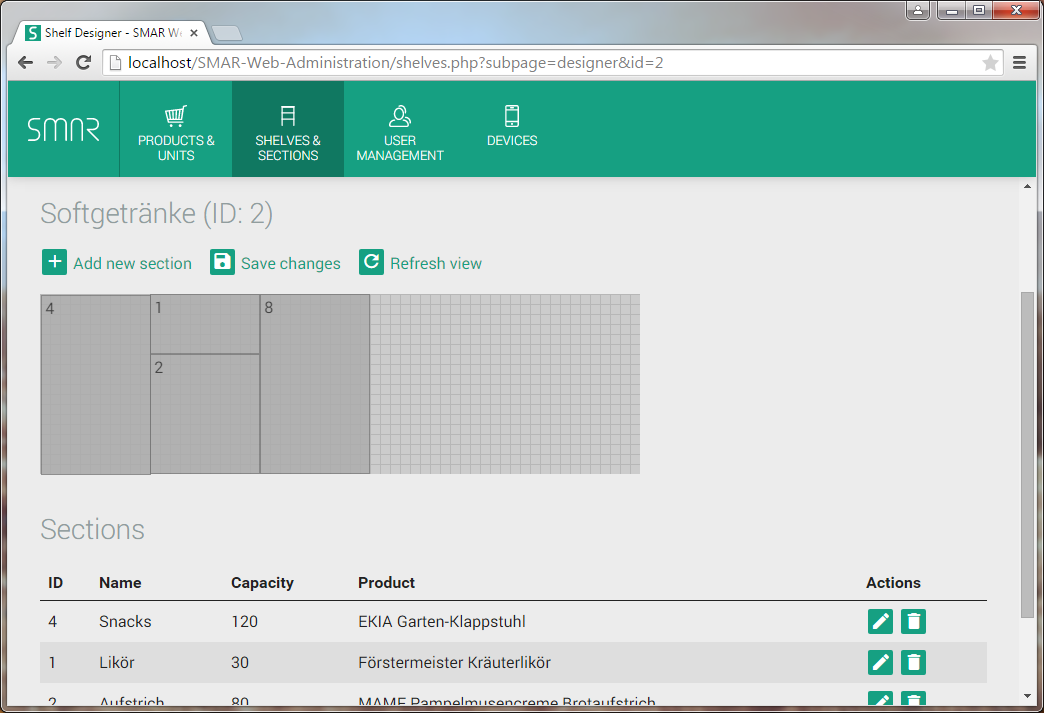
\includegraphics[width=\textwidth]{Bilder/Abbildungen/webadmin_shelves_designer.png}}
	\caption{Shelf Designer in der Webadministration (Screenshot)}
	\label{fig:webadmin_shelves_designer}
\end{figure}

Der Shelf Designer ist ein Tool in der \acs{SMAR} Webadministration, mit dessen Hilfe die Fächer eines Regals einfach angeordnet werden können. Wie in Abbildung \ref{fig:webadmin_shelves_designer} ersichtlich, besteht der Shelf Designer aus einer Arbeitsfläche, welche die Größe des zu bearbeitenden Regals hat. Auf der Arbeitsfläche sind die Regalfächer entsprechend ihrer in der Datenbank hinterlegten Position und Größe angeordnet.\\

Die Anordnung der Regalfächer kann per Drag \& Drop direkt verändert werden. Ebenso ist die Größenänderung durch Ziehen am Rahmen oder an den Ecken eines Fachs möglich. Auf dem Regal liegt dabei ein Grundraster mit einem Linienabstand von 10 Pixeln, wobei diese 10cm in Bezug auf die realen Maße des Regals entsprechen. Wird ein Regalfach bewegt oder in seiner Größe verändert, so ist dies nur entlang dieses Grundrasters möglich, alle Bewegungen rasten an den Grundlinien ein. Dadurch wird der Gestaltungsprozess für den Anwender deutlich vereinfacht. Um die Änderungen an der Regalanordnung letztendlich zu speichern, muss dieser nur auf Speichern drücken (\emph{Save changes}).\\

Neue Regalfächer lassen sich hier über einen Button anlegen. Im Gegensatz zu anderen Bereichen der Webadministration öffnet sich das Formular für eine neue  Section in einem Overlay, um den Arbeitsfluss mit dem Shelf Designer nicht zu unterbrechen. Im Formular muss zwingend ein verknüpftes Produkt eingegeben werden, welches dem Regalfach zugeordnet wird -- es muss also vorher ein Produkt zur Auswahl existieren. Nach Anlegen der neuen Section wird der Shelf Designer automatisch aktualisiert und enthält bereits die neue Section. Unter der Arbeitsfläche befindet sich eine Tabelle aller enthaltenen Regalfächer mit den üblichen Aktionen zum Bearbeiten und Löschen.\\


\subsection{Benutzerverwaltung}

%TODO Sebastian

\subsection{Weitere Funktionen}

Die für diese Arbeit vorliegende Version der \acs{SMAR} Webadministration enthält nur die notwendige Funktionalität, um die Grundfunktionen der App auf der Smartglass bedienen zu können. Das Datenbankschema ist jedoch schon für weitere Funktionen ausgelegt, die das Shelf Management mit \acs{SMAR} noch besser unterstützen und erweitern. Diese sollen im Folgenden kurz angeschnitten werden.

\subsubsection{Bestellungsmanagement}
Die Warenannahme bei neuen Produktlieferungen dient nicht nur dazu, die Produkte im Lager für das System zu erfassen. Durch die Prozessierung der Warenannahme sollen auch vorausgegangene Bestellungen dahingehend überprüft werden, ob die gelieferte Ware der Bestellliste entspricht. Auch sollen Differenzen in diesem Schritt erfasst und anschließend an den Lieferanten weitergegeben werden, sodass dieser nachliefern bzw. -buchen kann.\\

Um diese Prozesse abbilden zu können, müssen Bestellungen im System vorliegen. Diese sollen über die Webadministration angelegt und verwaltet werden können, dabei können die Positionen der Bestellung direkt aus den Produkten und Einheiten des Systems zusammengestellt werden, wodurch auch bei der Warenannahme durch die Smartglass keine weiteren Mappings der Bestellliste auf das System notwendig wären. Da verschiedene Einzelhandelsketten unterschiedliche interne Bestellsysteme verwenden und diese wahrscheinlich nicht direkt mit dem \acs{SMAR}-System kompatibel sind, muss außerdem eine Schnittstelle bereitgestellt werden, über welche Bestelldaten zwischen den Systemen transferiert werden können. Ebenso muss eine Differenzliste bei Lieferabweichungen im notwendigen Format bereit gestellt werden.

\subsubsection{Market Map}
Eine weitere praktische Zusatzfunktion des Systems wäre eine Wegfindung bzw. Navigation über die Verkaufsfläche, die z.B. beim Einräumen mehrerer Produkte hilfreich sein könnte, um eine optimale Route von Regal zu Regal zu berechnen. Dafür ist Voraussetzung, dass die Beschaffenheit der Verkaufsfläche mit allen Regalen und ihren Positionen bekannt ist.\\

Für diesen Zweck soll die Filiale über die Webadministration als \emph{Market Map} angelegt werden können. Diese definiert die Maße der Verkaufsfläche sowie die Regalpositionen und -ausrichtungen. Dazu bietet sich eine Umsetzung ähnlich dem Shelf Designer als eingebettetes Tool an (Map Designer). Ist die Verkaufsfläche auf diese Weise definiert, kann diese mit geringem technischem Aufwand zur Wegfindung verwendet werden.

